% Unit circle
% Original Author: Supreme Aryal
  % Licensed under https://creativecommons.org/licenses/by/2.5/
  % Found at http://www.texample.net/tikz/examples/unit-circle/
% Adapted by: Steven Clontz <http://clontz.org>
  % Licensed under https://creativecommons.org/licenses/by/2.5/

\documentclass{article}
\pagenumbering{gobble}
\usepackage{tikz}
\usepackage[top=1in,bottom=1in,right=1in,left=1in]{geometry}
\title{The Unit Circle}
\author{Prof. Steven Clontz}
\date{Last updated \today}


\begin{document}

\maketitle
Adapted from the original by Supreme Aryal at
http://www.texample.net/tikz/examples/unit-circle/

\vspace{1em}

Licensed under
https://creativecommons.org/licenses/by/2.5/

\vspace{1em}

http://clontz.org

\newpage


\begin{center}
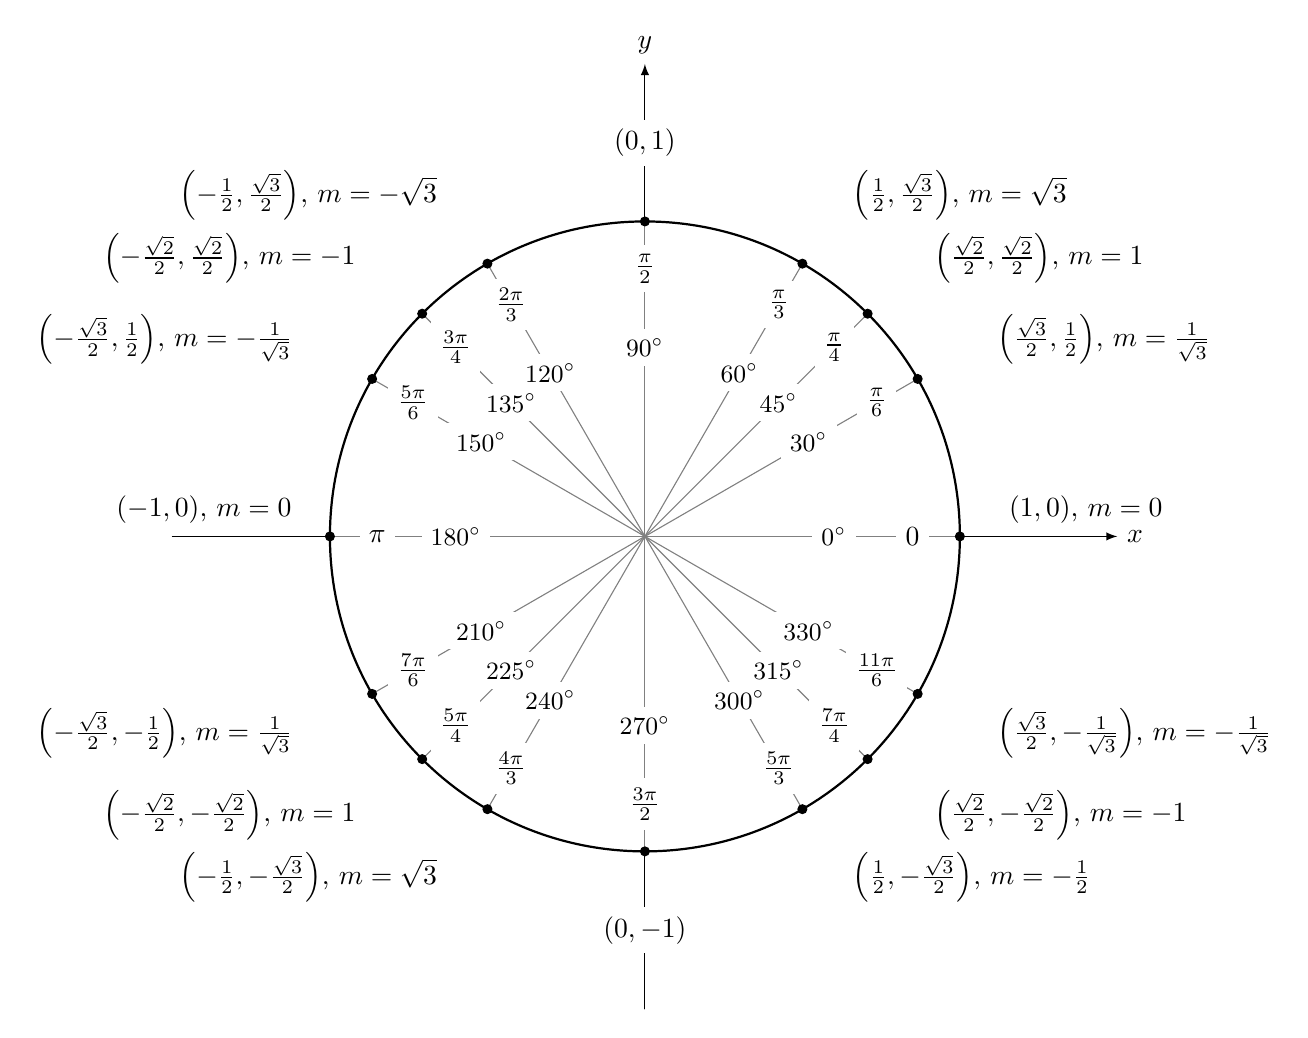
\begin{tikzpicture}[scale=4,cap=round,>=latex]
    % draw the coordinates
    \draw[->] (-1.5cm,0cm) -- (1.5cm,0cm) node[right,fill=white] {$x$};
    \draw[->] (0cm,-1.5cm) -- (0cm,1.5cm) node[above,fill=white] {$y$};

    % draw the unit circle
    \draw[thick] (0cm,0cm) circle(1cm);

    \foreach \x in {0,30,...,330} {
            % lines from center to point
            \draw[gray] (0cm,0cm) -- (\x:1cm);
            % dots at each point
            \filldraw[black] (\x:1cm) circle(0.4pt);
            % draw each angle in degrees
            \draw (\x:0.6cm) node[fill=white] {\small$\x^\circ$};
    }

    \foreach \x in {45,135,225,315} {
            % lines from center to point
            \draw[gray] (0cm,0cm) -- (\x:1cm);
            % dots at each point
            \filldraw[black] (\x:1cm) circle(0.4pt);
            % draw each angle in degrees
            \draw (\x:0.6cm) node[fill=white] {\small$\x^\circ$};
    }

    % draw each angle in radians
    \foreach \x/\xtext in {
        30/\frac{\pi}{6},
        45/\frac{\pi}{4},
        60/\frac{\pi}{3},
        90/\frac{\pi}{2},
        120/\frac{2\pi}{3},
        135/\frac{3\pi}{4},
        150/\frac{5\pi}{6},
        180/\pi,
        210/\frac{7\pi}{6},
        225/\frac{5\pi}{4},
        240/\frac{4\pi}{3},
        270/\frac{3\pi}{2},
        300/\frac{5\pi}{3},
        315/\frac{7\pi}{4},
        330/\frac{11\pi}{6},
        0/0}
            \draw (\x:0.85cm) node[fill=white] {$\xtext$};

    \foreach \x/\xtext/\y/\z in {
        % the coordinates for the second quadrant
        150/-\frac{\sqrt{3}}{2}/\frac{1}{2}/-\frac{1}{\sqrt{3}},
        135/-\frac{\sqrt{2}}{2}/\frac{\sqrt{2}}{2}/-1,
        120/-\frac{1}{2}/\frac{\sqrt{3}}{2}/-\sqrt{3},
        % the coordinates for the third quadrant
        210/-\frac{\sqrt{3}}{2}/-\frac{1}{2}/\frac{1}{\sqrt{3}},
        225/-\frac{\sqrt{2}}{2}/-\frac{\sqrt{2}}{2}/1,
        240/-\frac{1}{2}/-\frac{\sqrt{3}}{2}/\sqrt{3}}
            \draw (\x:1.25cm) node[fill=white,left=0.5pt] {$\left(\xtext,\y\right)$, $m=\z$};

    \foreach \x/\xtext/\y/\z in {
        % the coordinates for the first quadrant
        30/\frac{\sqrt{3}}{2}/\frac{1}{2}/\frac{1}{\sqrt{3}},
        45/\frac{\sqrt{2}}{2}/\frac{\sqrt{2}}{2}/1,
        60/\frac{1}{2}/\frac{\sqrt{3}}{2}/\sqrt{3},
        % the coordinates for the fourth quadrant
        330/\frac{\sqrt{3}}{2}/-\frac{1}{\sqrt{3}},
        315/\frac{\sqrt{2}}{2}/-\frac{\sqrt{2}}{2}/-1,
        300/\frac{1}{2}/-\frac{\sqrt{3}}{2}/-\frac{1}{2}/-\sqrt{3}}
            \draw (\x:1.25cm) node[fill=white,right=0.5pt] {$\left(\xtext,\y\right)$, $m=\z$};

    % draw the horizontal and vertical coordinates
    % the placement is better this way
    \draw (-1.4cm,0cm) node[above=1pt] {$(-1,0)$, $m=0$}
          (1.4cm,0cm)  node[above=1pt] {$(1,0)$, $m=0$}
          (0cm,-1.25cm) node[fill=white] {$(0,-1)$}
          (0cm,1.25cm)  node[fill=white] {$(0,1)$};
\end{tikzpicture}
\end{center}

\noindent\textbf{How to Use}

\begin{itemize}
\item
The unit circle traces the points \((x,y)\)
satisfying \(x^2+y^2=1\) by letting
\(x=\cos\theta\) and \(y=\sin\theta\) for \(0\leq\theta\leq2\pi\).
\item
The slope \(m\) of the non-vertical lines from the origin to each
point is given by \(m=\frac{y}{x}=\tan\theta\).
\end{itemize}

\newpage


\begin{center}
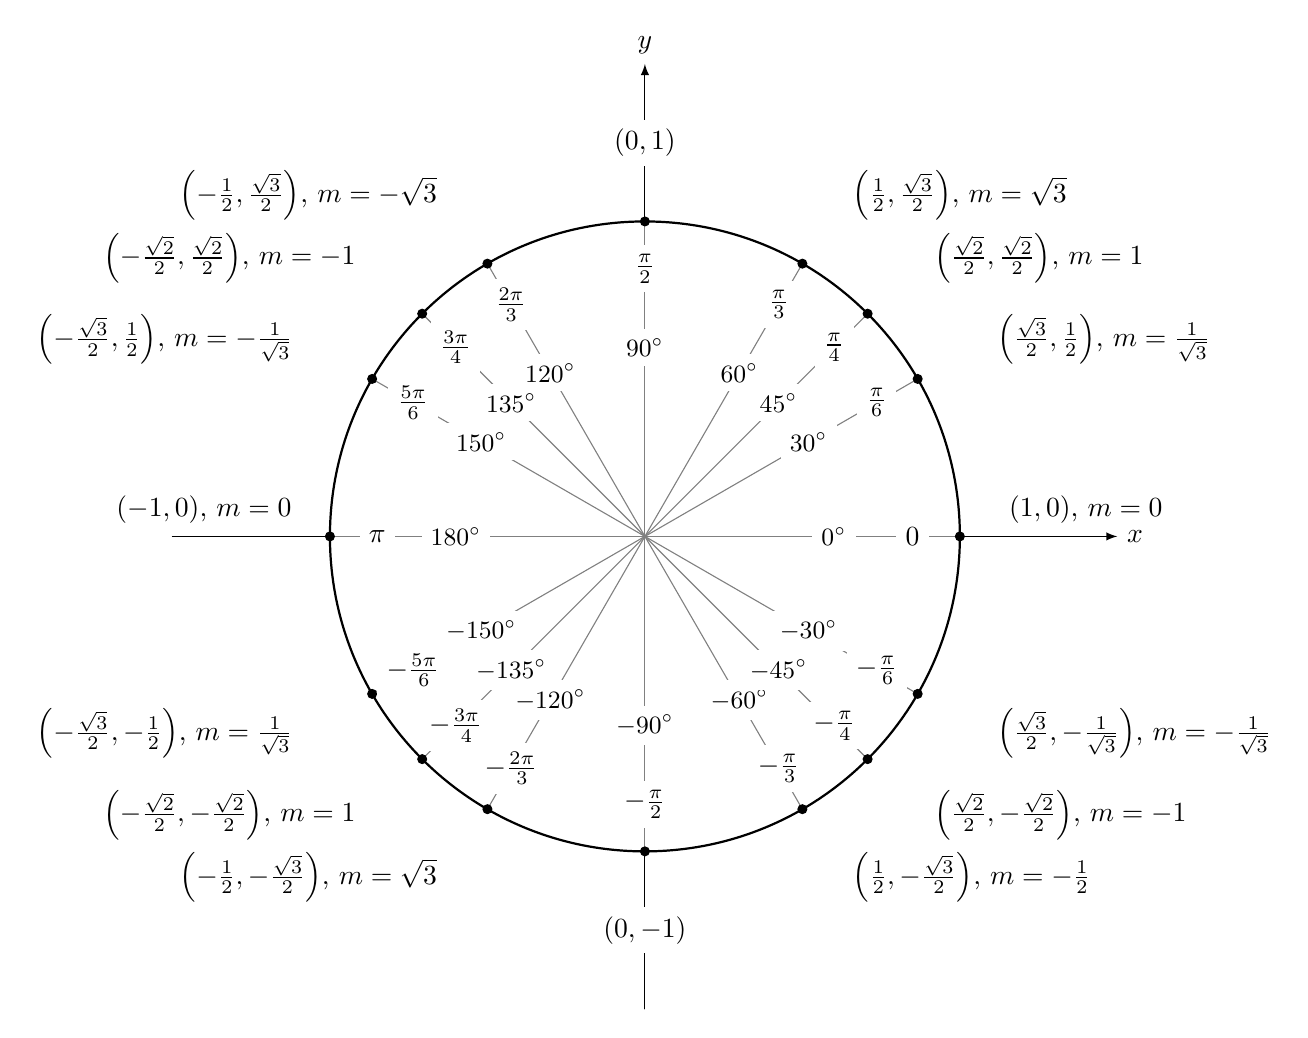
\begin{tikzpicture}[scale=4,cap=round,>=latex]
    % draw the coordinates
    \draw[->] (-1.5cm,0cm) -- (1.5cm,0cm) node[right,fill=white] {$x$};
    \draw[->] (0cm,-1.5cm) -- (0cm,1.5cm) node[above,fill=white] {$y$};

    % draw the unit circle
    \draw[thick] (0cm,0cm) circle(1cm);

    \foreach \x in {-150,-120,...,180} {
            % lines from center to point
            \draw[gray] (0cm,0cm) -- (\x:1cm);
            % dots at each point
            \filldraw[black] (\x:1cm) circle(0.4pt);
            % draw each angle in degrees
            \draw (\x:0.6cm) node[fill=white] {\small$\x^\circ$};
    }

    \foreach \x in {-135,-45,45,135} {
            % lines from center to point
            \draw[gray] (0cm,0cm) -- (\x:1cm);
            % dots at each point
            \filldraw[black] (\x:1cm) circle(0.4pt);
            % draw each angle in degrees
            \draw (\x:0.6cm) node[fill=white] {\small$\x^\circ$};
    }

    % draw each angle in radians
    \foreach \x/\xtext in {
        30/\frac{\pi}{6},
        45/\frac{\pi}{4},
        60/\frac{\pi}{3},
        90/\frac{\pi}{2},
        120/\frac{2\pi}{3},
        135/\frac{3\pi}{4},
        150/\frac{5\pi}{6},
        180/\pi,
        -150/-\frac{5\pi}{6},
        -135/-\frac{3\pi}{4},
        -120/-\frac{2\pi}{3},
        -90/-\frac{\pi}{2},
        -60/-\frac{\pi}{3},
        -45/-\frac{\pi}{4},
        -30/-\frac{\pi}{6},
        0/0}
            \draw (\x:0.85cm) node[fill=white] {$\xtext$};

    \foreach \x/\xtext/\y/\z in {
        % the coordinates for the second quadrant
        150/-\frac{\sqrt{3}}{2}/\frac{1}{2}/-\frac{1}{\sqrt{3}},
        135/-\frac{\sqrt{2}}{2}/\frac{\sqrt{2}}{2}/-1,
        120/-\frac{1}{2}/\frac{\sqrt{3}}{2}/-\sqrt{3},
        % the coordinates for the third quadrant
        210/-\frac{\sqrt{3}}{2}/-\frac{1}{2}/\frac{1}{\sqrt{3}},
        225/-\frac{\sqrt{2}}{2}/-\frac{\sqrt{2}}{2}/1,
        240/-\frac{1}{2}/-\frac{\sqrt{3}}{2}/\sqrt{3}}
            \draw (\x:1.25cm) node[fill=white,left=0.5pt] {$\left(\xtext,\y\right)$, $m=\z$};

    \foreach \x/\xtext/\y/\z in {
        % the coordinates for the first quadrant
        30/\frac{\sqrt{3}}{2}/\frac{1}{2}/\frac{1}{\sqrt{3}},
        45/\frac{\sqrt{2}}{2}/\frac{\sqrt{2}}{2}/1,
        60/\frac{1}{2}/\frac{\sqrt{3}}{2}/\sqrt{3},
        % the coordinates for the fourth quadrant
        330/\frac{\sqrt{3}}{2}/-\frac{1}{\sqrt{3}},
        315/\frac{\sqrt{2}}{2}/-\frac{\sqrt{2}}{2}/-1,
        300/\frac{1}{2}/-\frac{\sqrt{3}}{2}/-\frac{1}{2}/-\sqrt{3}}
            \draw (\x:1.25cm) node[fill=white,right=0.5pt] {$\left(\xtext,\y\right)$, $m=\z$};

    % draw the horizontal and vertical coordinates
    % the placement is better this way
    \draw (-1.4cm,0cm) node[above=1pt] {$(-1,0)$, $m=0$}
          (1.4cm,0cm)  node[above=1pt] {$(1,0)$, $m=0$}
          (0cm,-1.25cm) node[fill=white] {$(0,-1)$}
          (0cm,1.25cm)  node[fill=white] {$(0,1)$};
\end{tikzpicture}
\end{center}

\noindent\textbf{How to Use}

\begin{itemize}
\item
The unit circle traces the points \((x,y)\)
satisfying \(x^2+y^2=1\) by letting
\(x=\cos\theta\) and \(y=\sin\theta\) for \(-\pi\leq\theta\leq\pi\).
\item
The slope \(m\) of the non-vertical lines from the origin to each
point is given by \(m=\frac{y}{x}=\tan\theta\).
\end{itemize}
\end{document}
